\documentclass[usenames,dvipsnames,aspectratio=32]{beamer}
\usepackage[utf8]{inputenc}
\usecolortheme{seahorse}
\usepackage{amsmath,xfrac,dsfont,amsfonts,bbm,cancel,euler,ulem}
\usepackage{apacite,natbib}
\usepackage{hyperref}
\usepackage{caption,subcaption,booktabs,multicol,adjustbox}
\usepackage{xcolor,enumitem}

\setbeamercolor{section in toc}{fg=violet}
\setbeamercolor{subsection in toc}{fg=violet}

\title{The Missing ``Missing Middle'' \\ \small{Applied Macroeconomics: Micro Data for Macro Models} }
\author{Author: Chang-Tai Hsieh \and Benjamin A. Olken \\ Presented by: Jose M. Quintero}

\newcommand{\thus}{$\textcolor{violet}{\Longrightarrow}$}

\AtBeginSection[]
{
  \begin{frame}<beamer>
    \frametitle{Outline}
    \tableofcontents[currentsection]
  \end{frame}
}

\AtBeginSubsection[]
{
   \begin{frame}
        \frametitle{Outline}
        \tableofcontents[currentsubsection]
   \end{frame}
}



\begin{document}

\begin{frame}
  \titlepage
\end{frame}

\begin{frame}{Motivation}
    \begin{itemize}[label=\textcolor{violet}{$\blacktriangleright$}]
        \item \underline{The Missing Middle}: Few medium-size firms in developing countries relative to small and large firms. 
        \vfill
        \item Two prevailing theories:
        \begin{enumerate}[label=\textbf{\textcolor{violet}{\arabic*.}}]
            \item Small firms are disfavor by institutional setting $\textcolor{violet}{\Longrightarrow}$ Hard for small firms to grow.
            \item The burden of regulation is heavier on big firms $\textcolor{violet}{\Longrightarrow}$ Only very productive firms can overcome regulations. 
        \end{enumerate}
        \vfill 
        \item This Paper: Challenges the existence ``Missing Middle.''
        \begin{enumerate}[label=\textbf{\textcolor{violet}{\arabic*.}}]
            \item Test the implications of existing theories using Micro-data
            \item Why do we observe the ``Missing Middle''? 
        \end{enumerate}     
    \end{itemize}
\end{frame}

\begin{frame}{Main Results}
    \begin{enumerate}[label=\textbf{\textcolor{violet}{\arabic*.}}]
        \item There is no ``Missing Middle'' in the firm size distribution
        \begin{itemize}[label=\textcolor{violet}{$\blacktriangleright$}]
            \item Firm size distribution is not bimodal $\textcolor{violet}{\Longrightarrow}$ Big firms are also absent.
            \item Employment share \textcolor{violet}{+} Binning $\textcolor{violet}{\Longrightarrow}$ The ``Missing Middle'' 
            \item Size-dependent distortions barely generate bunching. 
        \end{itemize}
        \vfill
        \item Microdata does not favor constrained small firms:
        \begin{itemize}[label=\textcolor{violet}{$\blacktriangleright$}]
            \item No bimodality in the distribution of average return to inputs. 
            \item Marginal return to capital is higher for larger firms. 
        \end{itemize}            
        \vfill
        \item Data favors that the burden of regulation is heavier on big firms
        \begin{itemize}[label=\textcolor{violet}{$\blacktriangleright$}]
            \item Results may vary upon underlying technology assumption. 
        \end{itemize}
    \end{enumerate}
\end{frame}

\section{Existing Theories}

\begin{frame}{Disfavored Small Firms}
    \begin{itemize}[label=\textcolor{violet}{$\blacktriangleright$}]
        \item Institutional setting disfavor small firms. 
        \begin{itemize}[label=\textcolor{violet}{\small{$\blacktriangleright$}}]
            \item Credit constrained, financial access,
            \item Property rights are better protected for formal, 
            \item Policies favor big firms. 
        \end{itemize}
        \vfill
        \item Empirical Predictions
        \begin{enumerate}[label=\textbf{\textcolor{violet}{\arabic*.}}]
            \item Small and big firms are unconstrained \thus Marginal return to inputs is low. 
            \item ``Missing'' mid-size firms are constrained \thus Marginal return to inputs are high. 
            \item Bimodal distribution of marginal returns to inputs. 
        \end{enumerate}
    \end{itemize}
\end{frame}

\begin{frame}{A Dual Economy}
    \begin{itemize}[label=\textcolor{violet}{$\blacktriangleright$}]
        \item Medium and large firms face costs that small firms do not face. 
        \begin{enumerate}[label=\textbf{\textcolor{violet}{\arabic*.}}]
            \item Mid-size firms cannot overcome the barriers \thus Remain small. 
            \item Ej: Size-dependent regulations, minimum wages, registration (fix costs). 
        \end{enumerate}
        \vfill
        \item Empirical Predictions
        \begin{enumerate}[label=\textbf{\textcolor{violet}{\arabic*.}}]
            \item Barbell shaped for returns to capital. 
            \item Returns to inputs by firm size are dependent on production technology. 
            \item Size-dependent distortions \thus Right skewed f.s.d + higher return for big firms. 
        \end{enumerate}
    \end{itemize}
\end{frame}

\section{Testing against the data}
\begin{frame}{Firm Size Distribution}
    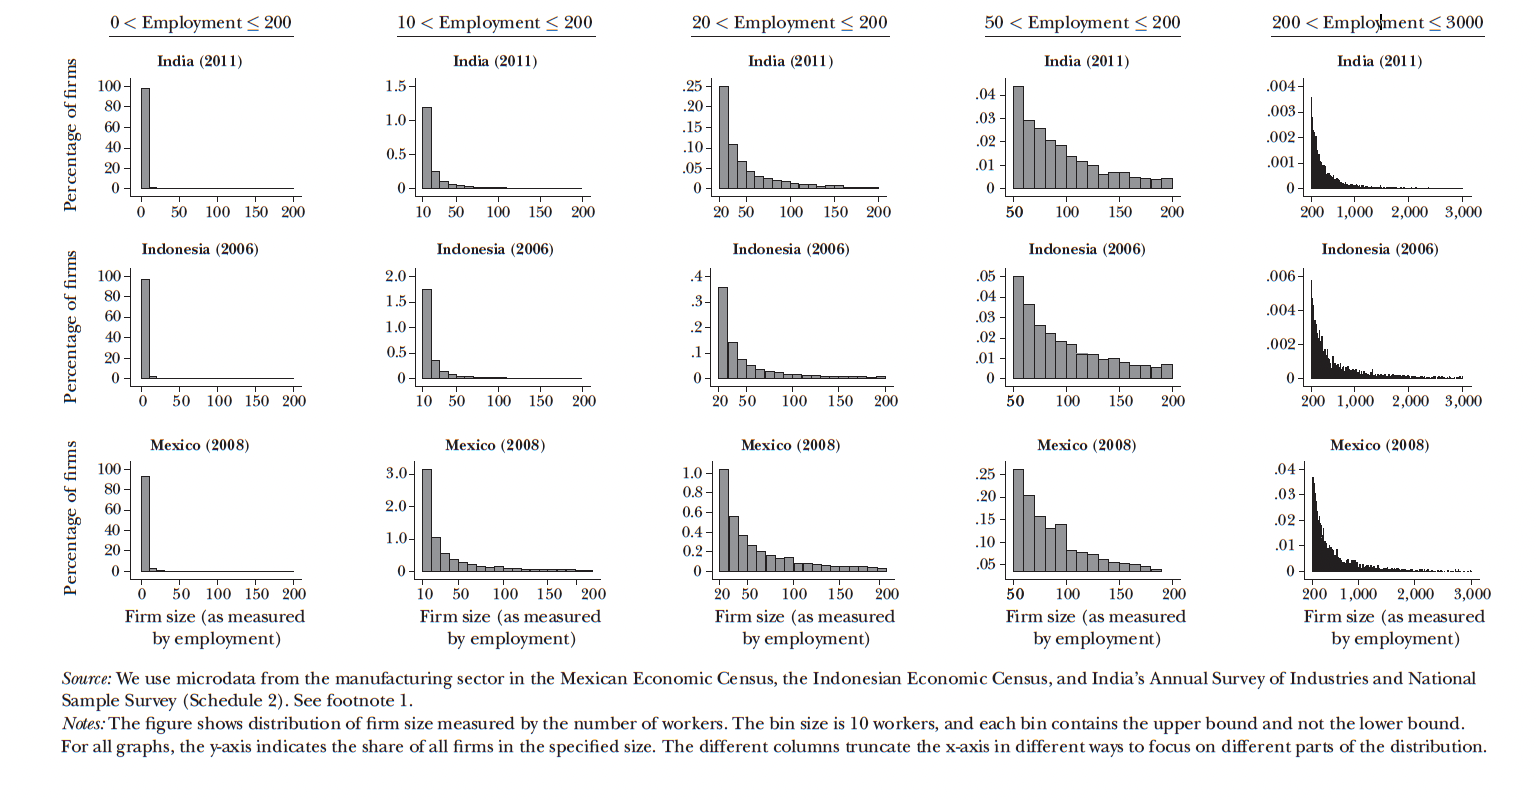
\includegraphics[width=\textwidth]{Figures/FirmSizeDist.png}
\end{frame}

\begin{frame}{Distribution of Average products}
\begin{center}
    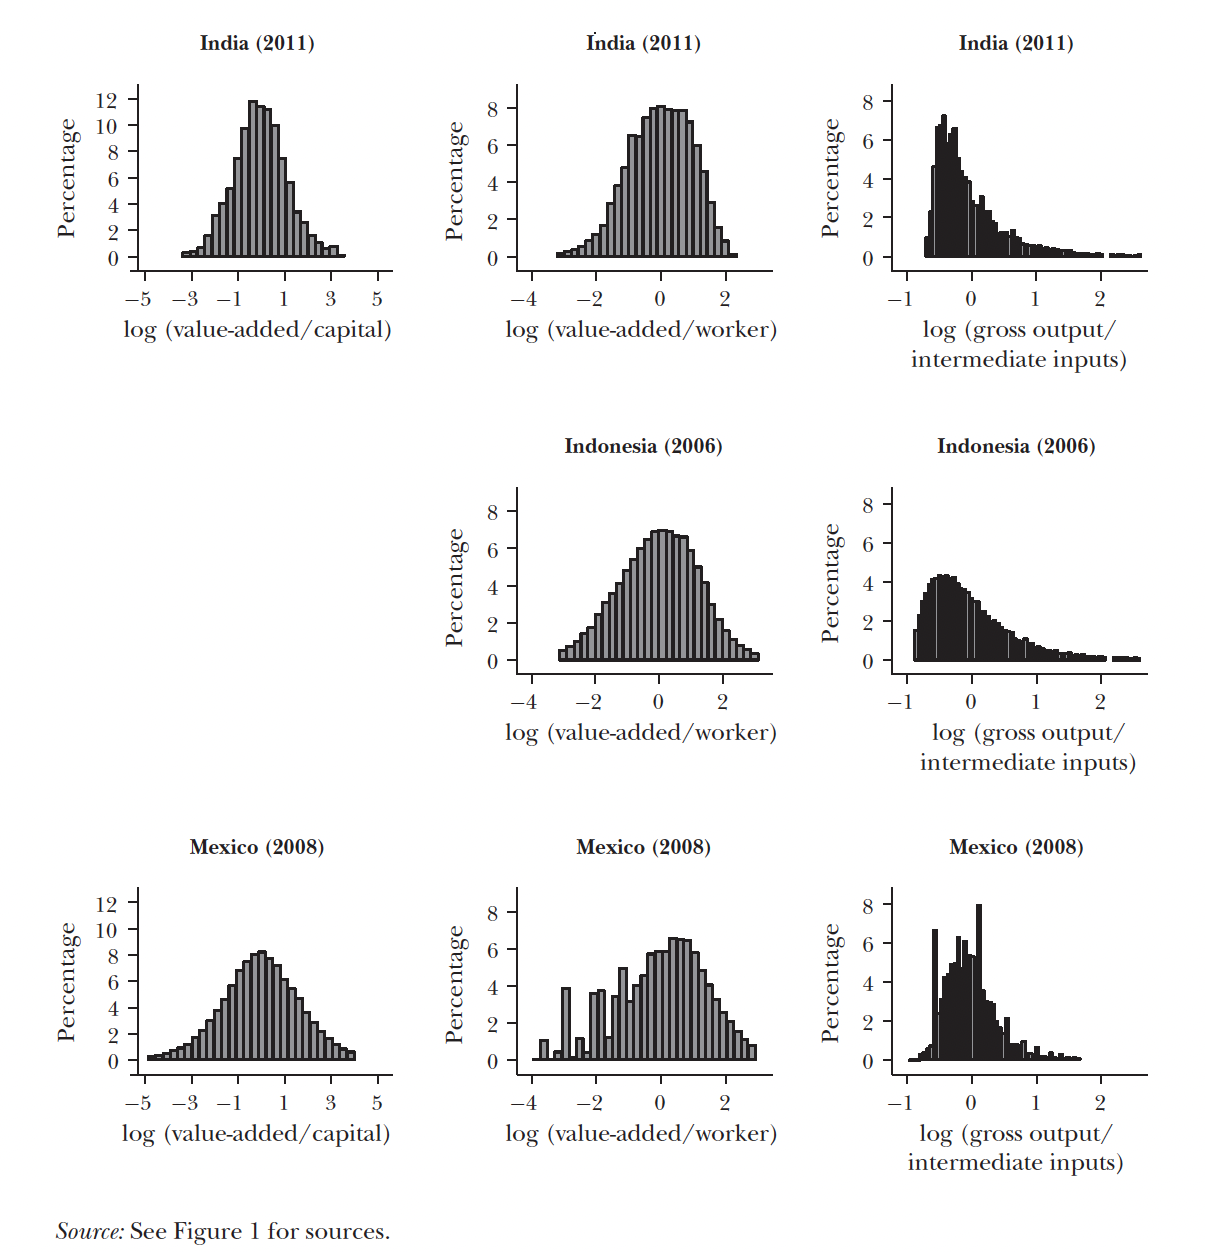
\includegraphics[width=0.65\textwidth]{Figures/ReturnDistribution.png}
\end{center}
\end{frame}

\begin{frame}{Average Product and Firm Size}
\begin{center}
    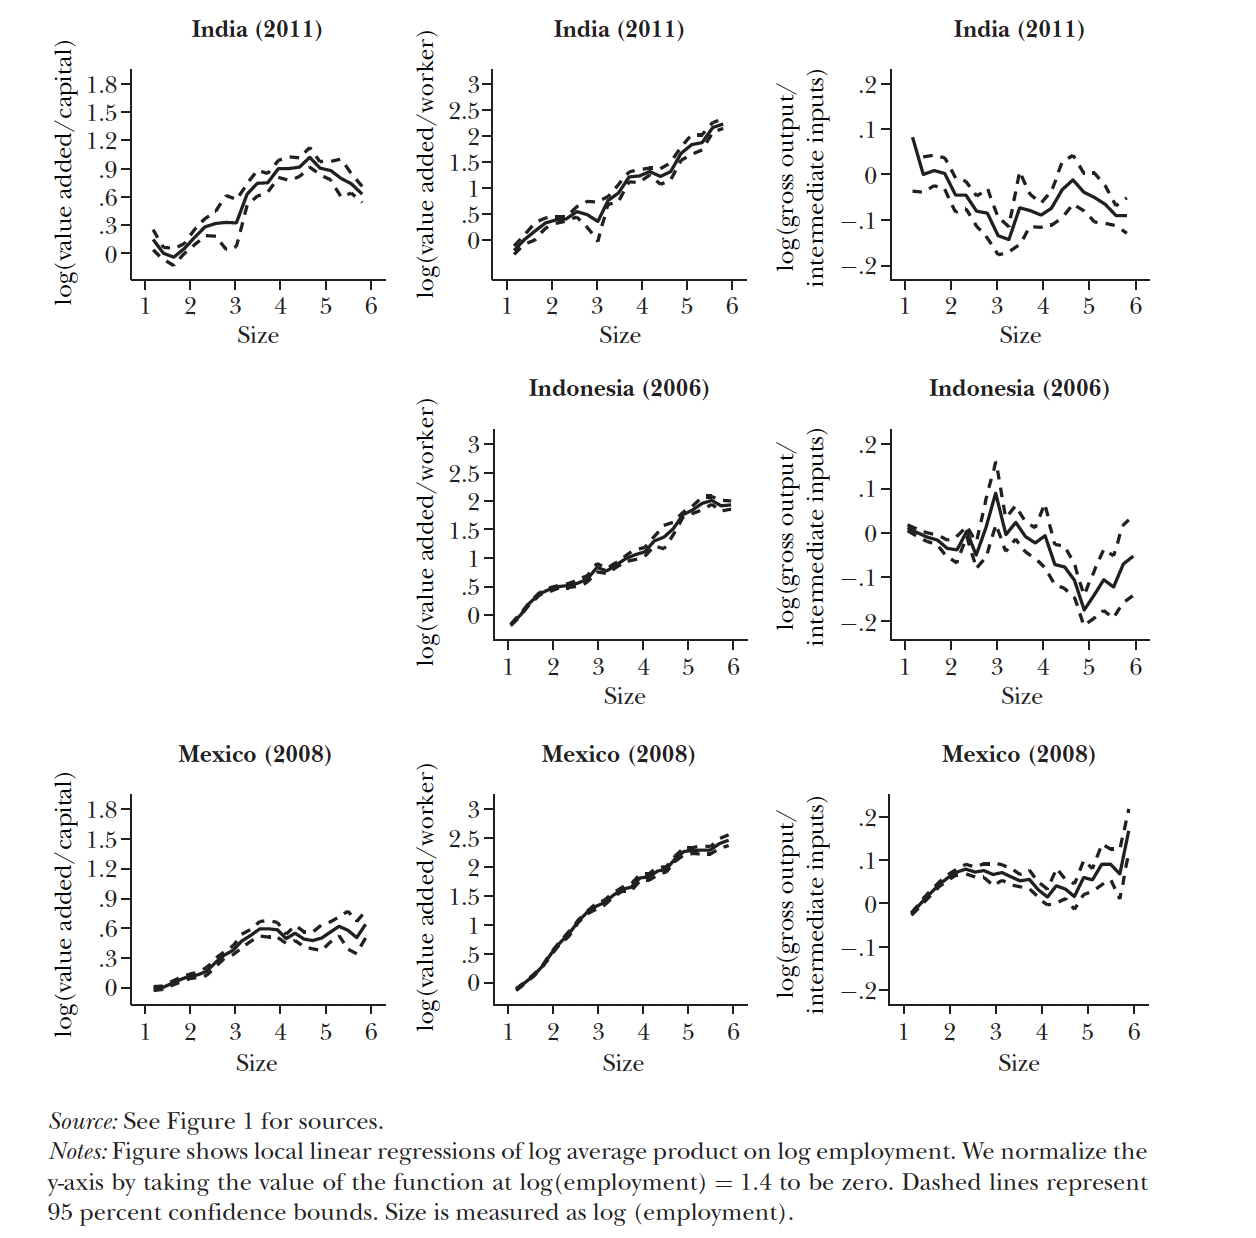
\includegraphics[width=0.65\textwidth]{Figures/ReturnFirmSize.png}
\end{center}
\end{frame}

\begin{frame}{Size-Dependent Distortions}
    \begin{enumerate}[label=\textbf{\textcolor{violet}{\arabic*.}}]
        \item Distortion in terms of employment
        \item Distortions in terms of 
    \end{enumerate}
\end{frame}

\begin{frame}{The case of Mexico}
    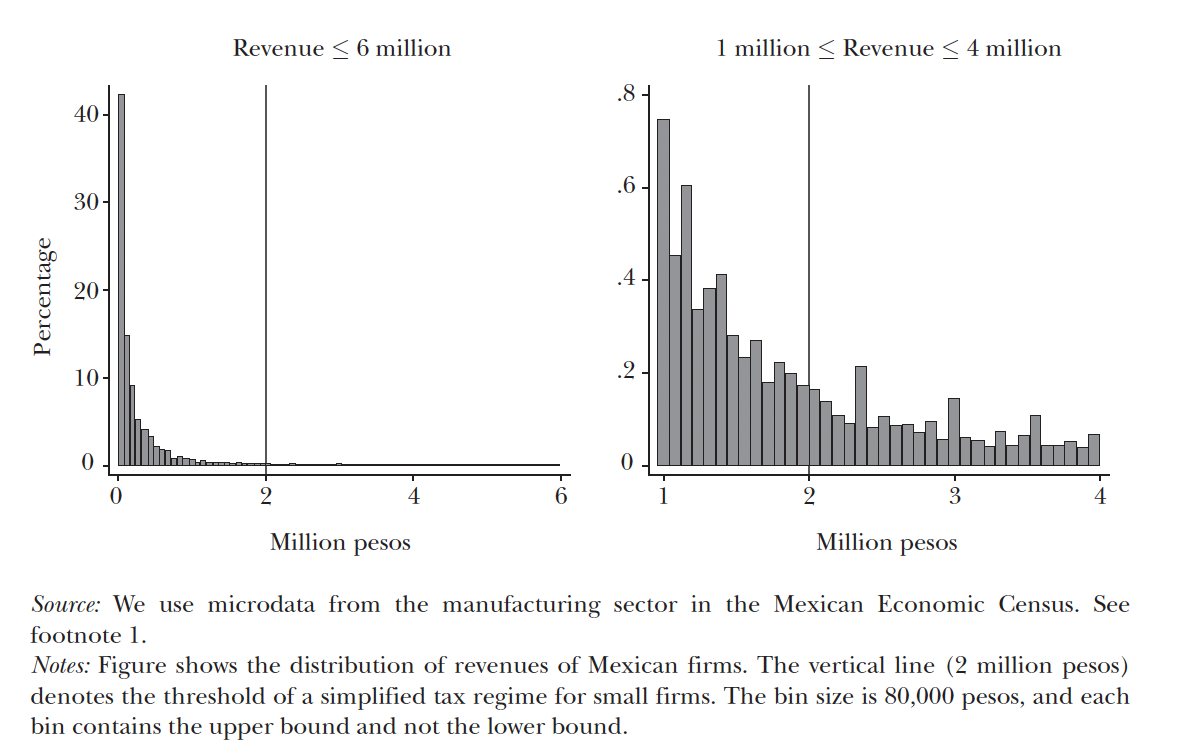
\includegraphics[width=\textwidth]{Figures/MexicoSizeDependent.png}
\end{frame}

\begin{frame}{The Case of India}{Informality}
    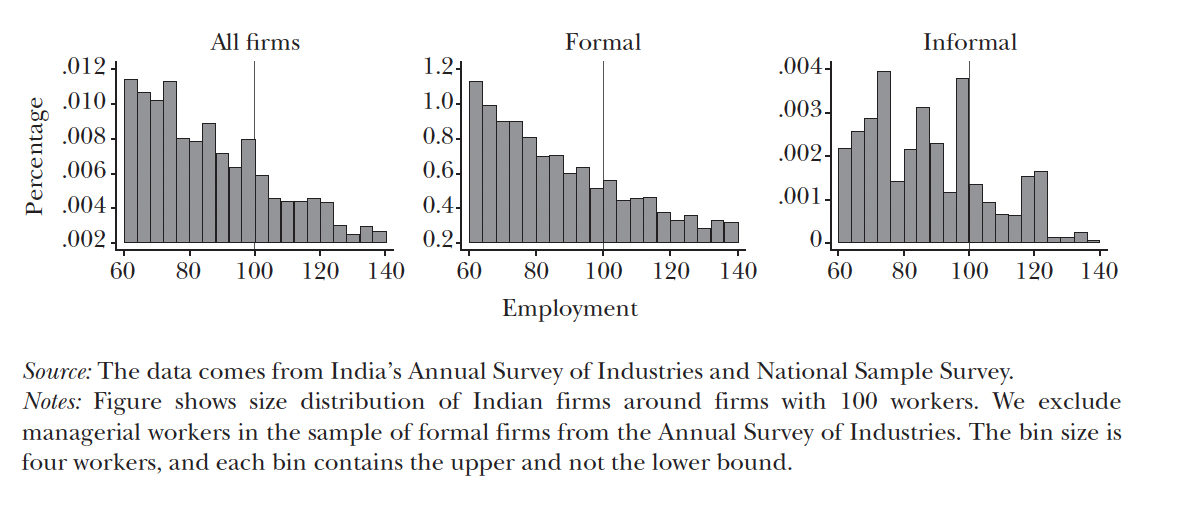
\includegraphics[width=\textwidth]{Figures/IndiaSizeDependent.png}
\end{frame}


\end{document}

